\documentclass[../notes.tex]{subfiles}

\pagestyle{main}
\renewcommand{\chaptermark}[1]{\markboth{\chaptername\ \thechapter\ (#1)}{}}
\setcounter{chapter}{13}

\begin{document}




\chapter{???}
\section{Kinetic Resolution and Related Asymmetric Processes}
\begin{itemize}
    \item \marginnote{12/3:}Announcements.
    \begin{itemize}
        \item Today: Last Tuesday's lecture.
        \begin{itemize}
            \item Next time: Electron Transfer.
        \end{itemize}
        \item Exam 2 tomorrow.
        \begin{itemize}
            \item Format like the practice exam.
            \item Administered remotely.
            \item Work alone, and closed note (honor code).
            \item Available for 48 hours: Start of Wednesday til end of Thursday.
        \end{itemize}
        \item Do the teaching evaluations for both Alex and Masha!!
    \end{itemize}
    \item Today: Kinetic selectivities.
    \item Consider a starting material (\ce{SM}) that can evolve to a product \ce{A} or \ce{B}.
    \begin{figure}[h!]
        \centering
        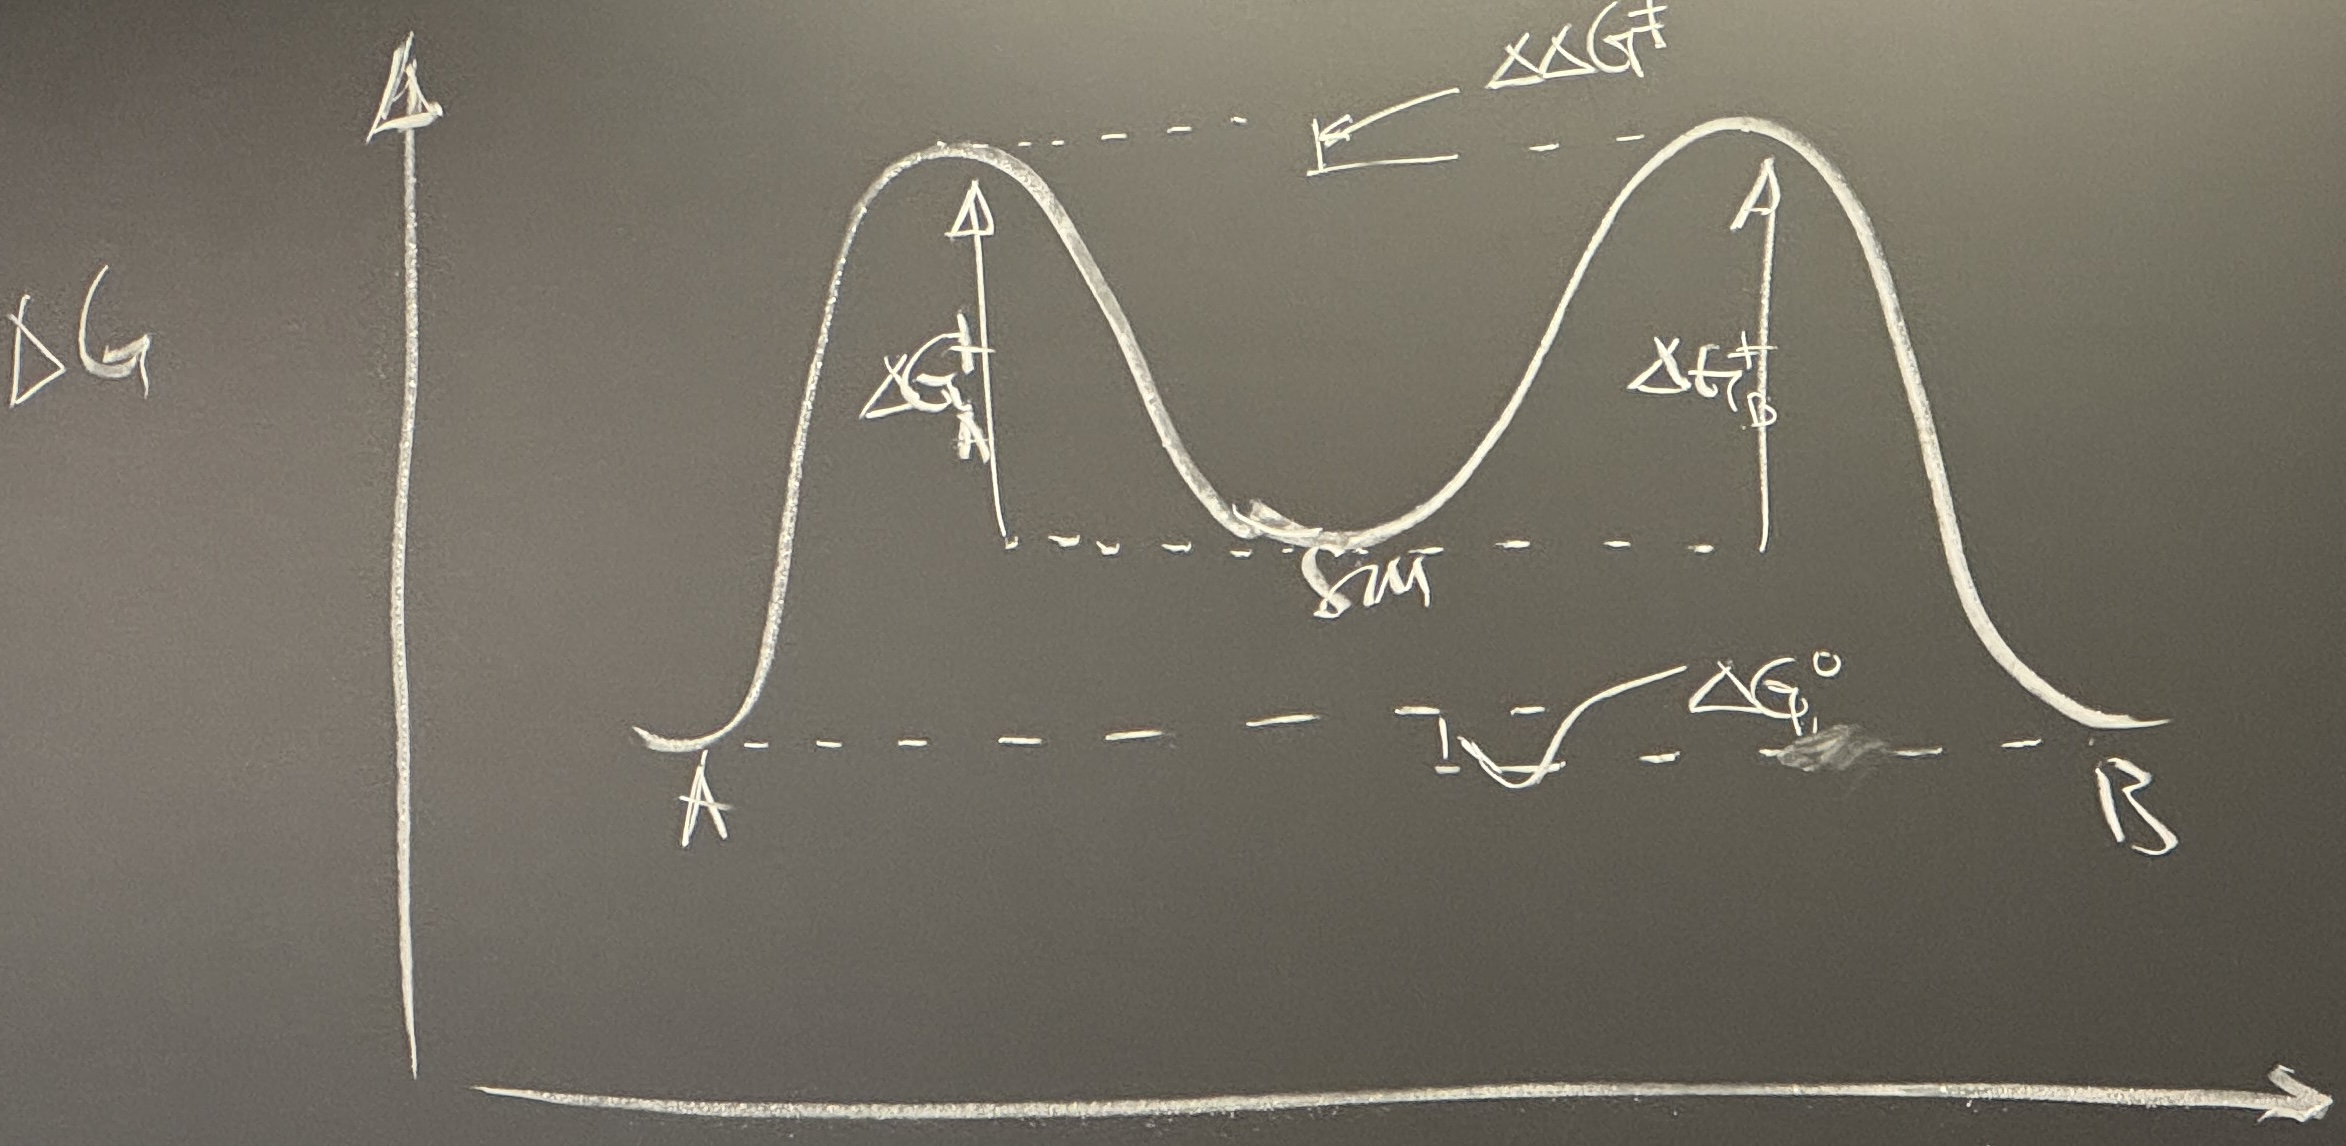
\includegraphics[width=0.55\linewidth]{selectThermKin.JPG}
        \caption{Thermodynamic vs. kinetic selectivity energy diagram.}
        \label{fig:selectThermKin}
    \end{figure}
    \begin{itemize}
        \item We can map this reaction onto a potential energy surface.
        \item If \ce{A} and \ce{B} are free to reversibly interconvert, then we can explain the product distribution in terms of the $\Delta G^\circ$ between \ce{A} and \ce{B}.
        \begin{itemize}
            \item In particular, $\Delta G=-RT\ln\Keq$ where $\Keq=\cnc{A}/\cnc{B}$.
        \end{itemize}
        \pagebreak
        \item Today, we'll consider the case in which \ce{A} and \ce{B} do \emph{not} reversibly interconvert.
        \begin{itemize}
            \item In this case, what's important is the $\Delta\Delta G^\ddagger$ between the transition states.
            \item Here, the selectivity is given as the ratio of the rate constants:
            \begin{equation*}
                \text{selectivity} = \frac{\cnc{A}}{\cnc{B}}
                = \frac{k_{\ce{A}}}{k_{\ce{B}}}
                = \frac{\e[-\Delta G^\ddagger_{\ce{A}}/RT]}{\e[-\Delta G^\ddagger_{\ce{B}}/RT]}
                = \e[-\Delta\Delta G^\ddagger/RT]
            \end{equation*}
            \item Note that $k_{\ce{A}}/k_{\ce{B}}=\krel$. This quantity is important for determing dr's, er's, etc.
        \end{itemize}
    \end{itemize}
    \item A case in which kinetic selectivity is important: Catalytic kinetic resolution.
    \begin{figure}[h!]
        \centering
        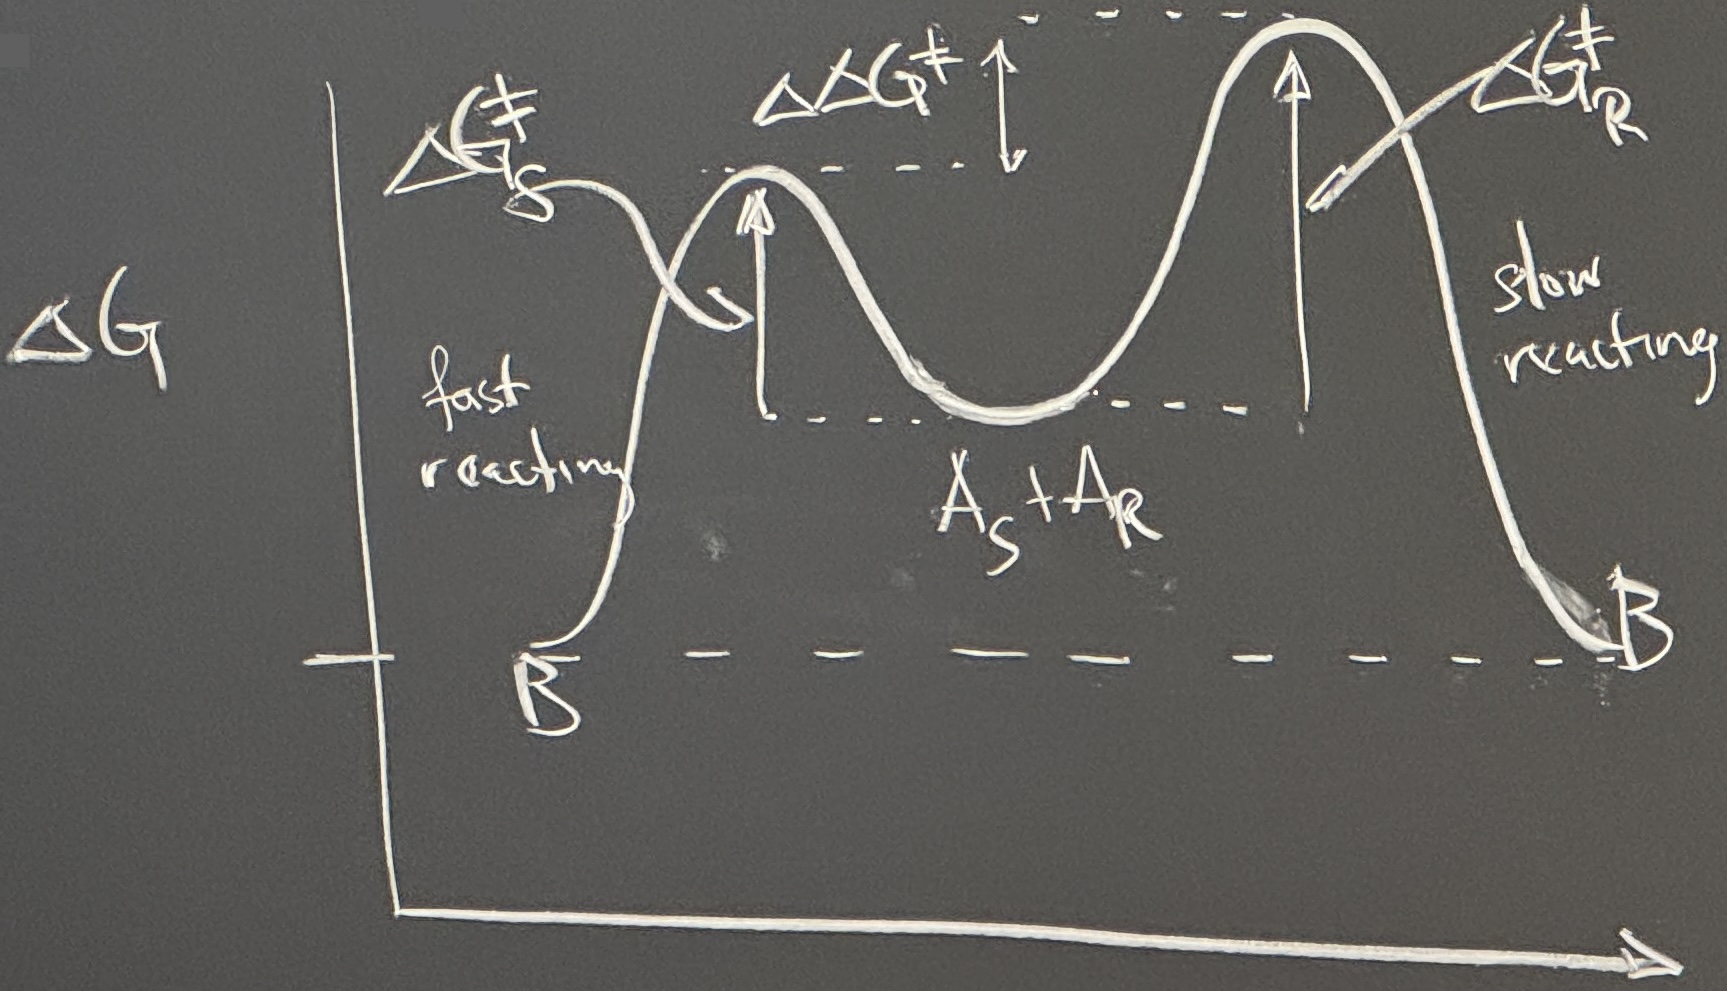
\includegraphics[width=0.4\linewidth]{EDcatKinRes.JPG}
        \caption{Catalytic kinetic resolution energy diagram.}
        \label{fig:EDcatKinRes}
    \end{figure}
    \begin{itemize}
        \item \ce{A} is our starting material, a chiral racemic compound.
        \begin{itemize}
            \item Thus, we can denote the starting materials as \ce{A_S + A_R}.
            \item As enantiomers, \ce{A_R} and \ce{A_S} have identical free energies.
        \end{itemize}
        \item \ce{cat^*} is a \textbf{homochiral} catalyst.
        \item Then resolution to a product \ce{B} can happen two different ways: Through a transition state that consumes the (\emph{S})-enantiomer, and through a transition state that consumes the (\emph{R})-enantiomer.
        \item When a homochiral catalyst acts on two enantiomers, it forms two different, diastereomeric adducts: \ce{A_S*cat^*} and \ce{A_R*cat^*}.
        \begin{itemize}
            \item Unlike enantiomers, diastereomers \emph{are} different compounds that may have two different energies.
        \end{itemize}
        \item What we've indicated in Figure \ref{fig:EDcatKinRes} is that the (\emph{S})-enantiomer is converted faster than the (\emph{R})-enantiomer.
        \item Thus,
        \begin{equation*}
            \krel = \frac{\kf}{\ks}
            = \e[-\Delta\Delta G^\ddagger/RT]
        \end{equation*}
        \begin{itemize}
            \item In the literature, $\krel$ is sometimes referred to as an \textbf{S-factor} (for "selectivity factor").
        \end{itemize}
        \item Reference: \textcite{bib:EDcatKinRes}.
    \end{itemize}
    \item \textbf{Homochiral} (catalyst): A chiral catalyst of which we're using only a single enantiomer.
    \item There are many catalytic kinetic resolutions in the literature.
    \begin{itemize}
        \item Radosevich developed one in grad school, when he was roughly our age!
    \end{itemize}
    \pagebreak
    \item Example catalytic kinetic resolution.
    \begin{figure}[h!]
        \centering
        \footnotesize
        \schemestart
            \chemname{
                \chemfig{*3([7](-Me)--O-)}
            }{($\pm$)}
            \+
            \chemname{
                \chemfig{H_2O}
            }{0.55 eq.}
            \arrow(.7--){->[0.2 mol\% (\emph{R},\emph{R})-\ce{(salen)Co^{III}(OAc)}][neat]}[,3.6]
            \chemnameinit{}
            \chemname{
                \chemfig{Me-[:15]*3(--O>:)}
            }{\tikz{\node[align=center]{44\% yield\\99\% ee};}}
            \+{,,0.7em}
            \chemname{
                \chemfig{Me-[:30](<[2]OH)-[:-30]-[:30]OH}
            }{\tikz{\node[align=center]{50\% yield\\98\% ee};}}
        \schemestop
        \caption{Hydrolytic kinetic resolution.}
        \label{fig:kinResHydro}
    \end{figure}
    \begin{itemize}
        \item Take propylene oxide (racemic) and 0.55 eq. of water.
        \item React them, neat, in the presence of a small amount of homochiral catalyst.
        \begin{itemize}
            \item The structure of this complex is totally irrelevant to our aims, but we can look it up in the reference if we're curious.
            \item This is our homochiral catalyst that will act on the two relatively inexpensive starting materials.
        \end{itemize}
        \item We run this reaction neat, and recover one enantiomer of our starting material in nearly quantitative yield with near perfect ee.
        \item We also obtain a ring-opened \emph{vic}-diol in nearly quantitative yield with near perfect ee.
        \item $\krel\approx 500$ here!
        \item Reference: \textcite{bib:kinResHydro}.
        \item This is a \textbf{hydrolytic kinetic resolution}.
        \begin{itemize}
            \item This is a very useful reaction for the resolution of terminal epoxides --- and access to terminal 1,2-diols --- because there exists no method to synthetically prefer a single enantiomer.
            \item Propylene is so small that even the best chiral epoxidation catalysts aren't very selective here, so it's better to do a racemic epoxidation and then this.
        \end{itemize}
        \item Great atom economy.
    \end{itemize}
    \item In a kinetic resolution like the above, the percent ee of both starting material and product is subject to change over time.
    \item To see this, let's build a theoretical model for a catalytic kinetic resolution.
    \begin{align*}
        \ce{A_S + cat^*} &\ce{->[$\kf$] P}&
        \ce{A_R + cat^*} &\ce{->[$\ks$] P}
    \end{align*}
    \begin{itemize}
        \item The net transformation involves the above two chemical reactions.
        \item We can write differential rate laws for each enantiomer
        \begin{align*}
            \dv{\cnc{A_S}}{t} &= -\kf\cnc{A_S}\cnc{cat^*}&
            \dv{\cnc{A_R}}{t} &= -\ks\cnc{A_R}\cnc{cat^*}
        \end{align*}
        \begin{itemize}
            \item The consumption of the fast-reaction enantiomer will deplete $\cnc{A}$.
        \end{itemize}
        \item Assuming $\cnc{cat^*}$ is approximately constant throughout the reaction, each of these differential rate laws can be independently integrated to
        \begin{align*}
            \ln(\frac{\cnc{A_S}}{\cnc[0]{A_S}}) &= -\kf\cnc{cat^*}t&
            \ln(\frac{\cnc{A_R}}{\cnc[0]{A_R}}) &= -\ks\cnc{cat^*}t
        \end{align*}
        \item Then, the key thing to note here is that for a racemic mixture, $\cnc[0]{A_S}=\cnc[0]{A_R}$.
        \item Thus, we can make this substitution and divide the above two integrated rate laws to get
        \begin{equation*}
            \krel = \frac{\kf}{\ks}
            = \frac{\ln(\cnc{A_S}/\cnc[0]{A_S})}{\ln(\cnc{A_R}/\cnc[0]{A_S})}
        \end{equation*}
    \end{itemize}
    \item This is a useful result, but we can make it even better. We'll start with a couple of definitions.
    \item \textbf{Conversion}: The ratio of how much of a reactant has reacted. \emph{Denoted by} $\bm{c}$. \emph{Given by}
    \begin{equation*}
        c := 1-\frac{\cnc{A_S}+\cnc{A_R}}{\cnc[0]{A_S}+\cnc[0]{A_R}}
        = 1-\frac{\cnc{A_S}+\cnc{A_R}}{2\cnc[0]{A_S}}
    \end{equation*}
    \item \textbf{Enantiomeric excess}: A measurement of the degree to which a sample contains one enantiomer in greater amounts than the other. \emph{Denoted by} \textbf{ee}. \emph{Given by}
    \begin{equation*}
        \text{ee} := \frac{\cnc{A_S}-\cnc{A_R}}{\cnc{A_S}+\cnc{A_R}}
    \end{equation*}
    \item We can now do some algebra.
    \begin{itemize}
        \item Indeed, it follows from the above definitions that
        \begin{align*}
            1-\text{ee} &= \frac{2\cnc{A_R}}{\cnc{A_S}+\cnc{A_R}}&
            1+\text{ee} &= \frac{2\cnc{A_S}}{\cnc{A_S}+\cnc{A_R}}
        \end{align*}
        \item Then we can derive the following interesting relatinoships.
        \begin{align*}
            \frac{\cnc{A_R}}{\cnc[0]{A_S}} &= (1-c)(1-ee)&
            \frac{\cnc{A_S}}{\cnc[0]{A_S}} &= (1-c)(1+ee)
        \end{align*}
        \item We can now know the extent to which a reaction has evolved to consume one enantiomer or the other as a function of observables!
    \end{itemize}
    \item Thus, we may define $\text{S}=\krel$ as a function of conversion and ee.
    \begin{itemize}
        \item For recovered starting material,
        \begin{equation*}
            \text{S} = \frac{\ln[(1-c)(1-ee)]}{\ln[(1-c)(1+ee)]}
        \end{equation*}
        \item For the product,
        \begin{equation*}
            \text{S} = \frac{\ln[(1-c)(1+ee)]}{\ln[(1-c)(1-ee)]}
        \end{equation*}
    \end{itemize}
    \item These relations allow us to relate conversion to ee for a catalyst of a given, set selectivity S. Specifically, we can parametrically plot ee as a function of conversion.
    \item Let's first do this for the percent ee in the recovered starting material.
    \begin{figure}[H]
        \centering
        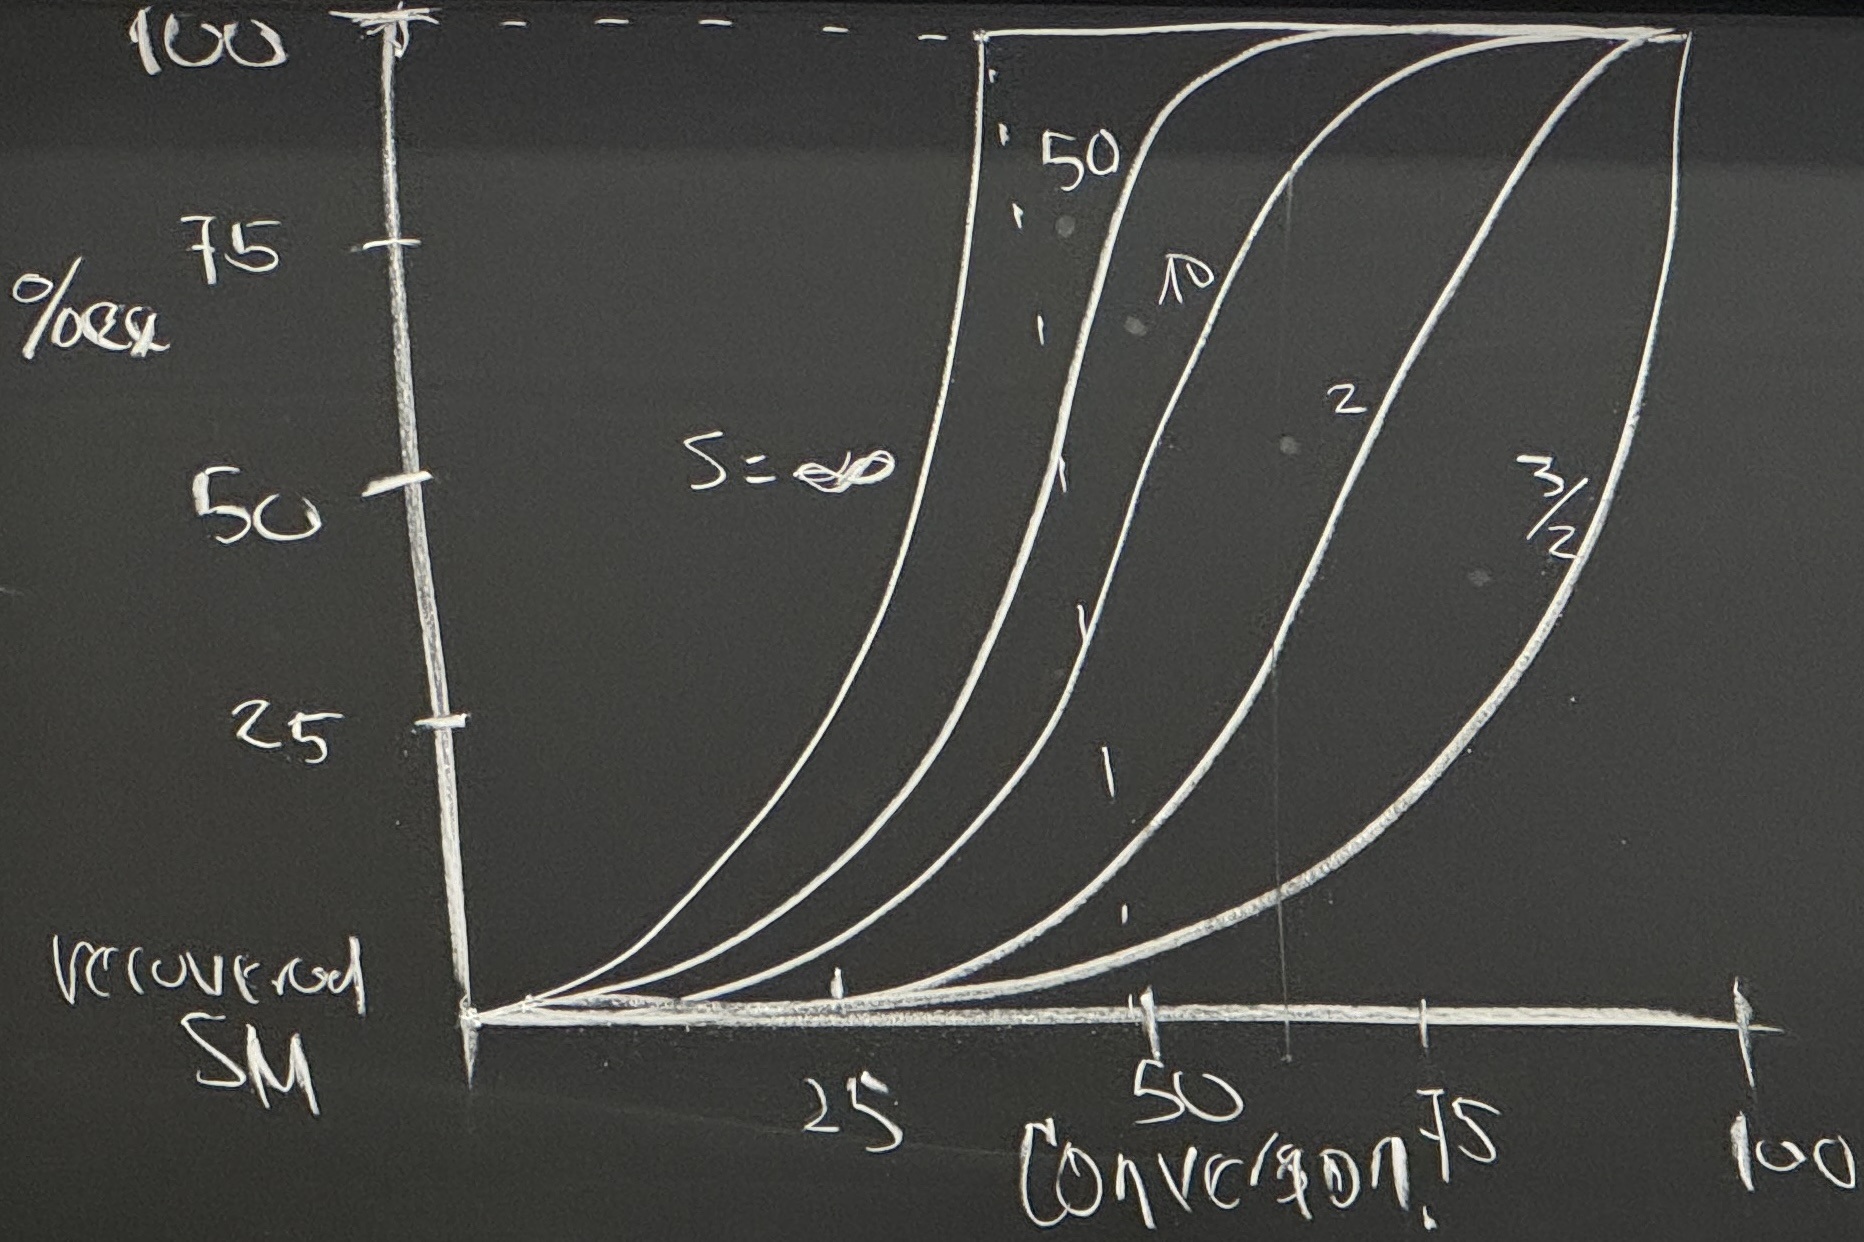
\includegraphics[width=0.45\linewidth]{kinResSMee.JPG}
        \caption{Starting material ee vs. conversion in a catalytic kinetic resolution.}
        \label{fig:kinResSMee}
    \end{figure}
    \begin{itemize}
        \item Consider first what happens in the limit that our selectivity factor is very large, i.e., that $\Delta\Delta G^\ddagger=\text{large}$.
        \item If $S=\infty$, then 50\% conversion will get us all we need.
        \begin{itemize}
            \item This is because at this point, the enantiomer we don't want to recover will have been fully consumed.
        \end{itemize}
        \item As the S-factor drops, we need higher conversions to get better ee's in the recovered starting material.
        \item What's cool about this is we can still get high ee's with bad catalysts\dots at the expense of conversion.
        \begin{itemize}
            \item Essentially, with bad catalysts, we'll recover \emph{less} enantiopure starting material (because some of it will have been consumed at higher conversions), but we \emph{can} still recover essentially enantiopure starting material.
        \end{itemize}
    \end{itemize}
    \item For the product.
    \begin{figure}[h!]
        \centering
        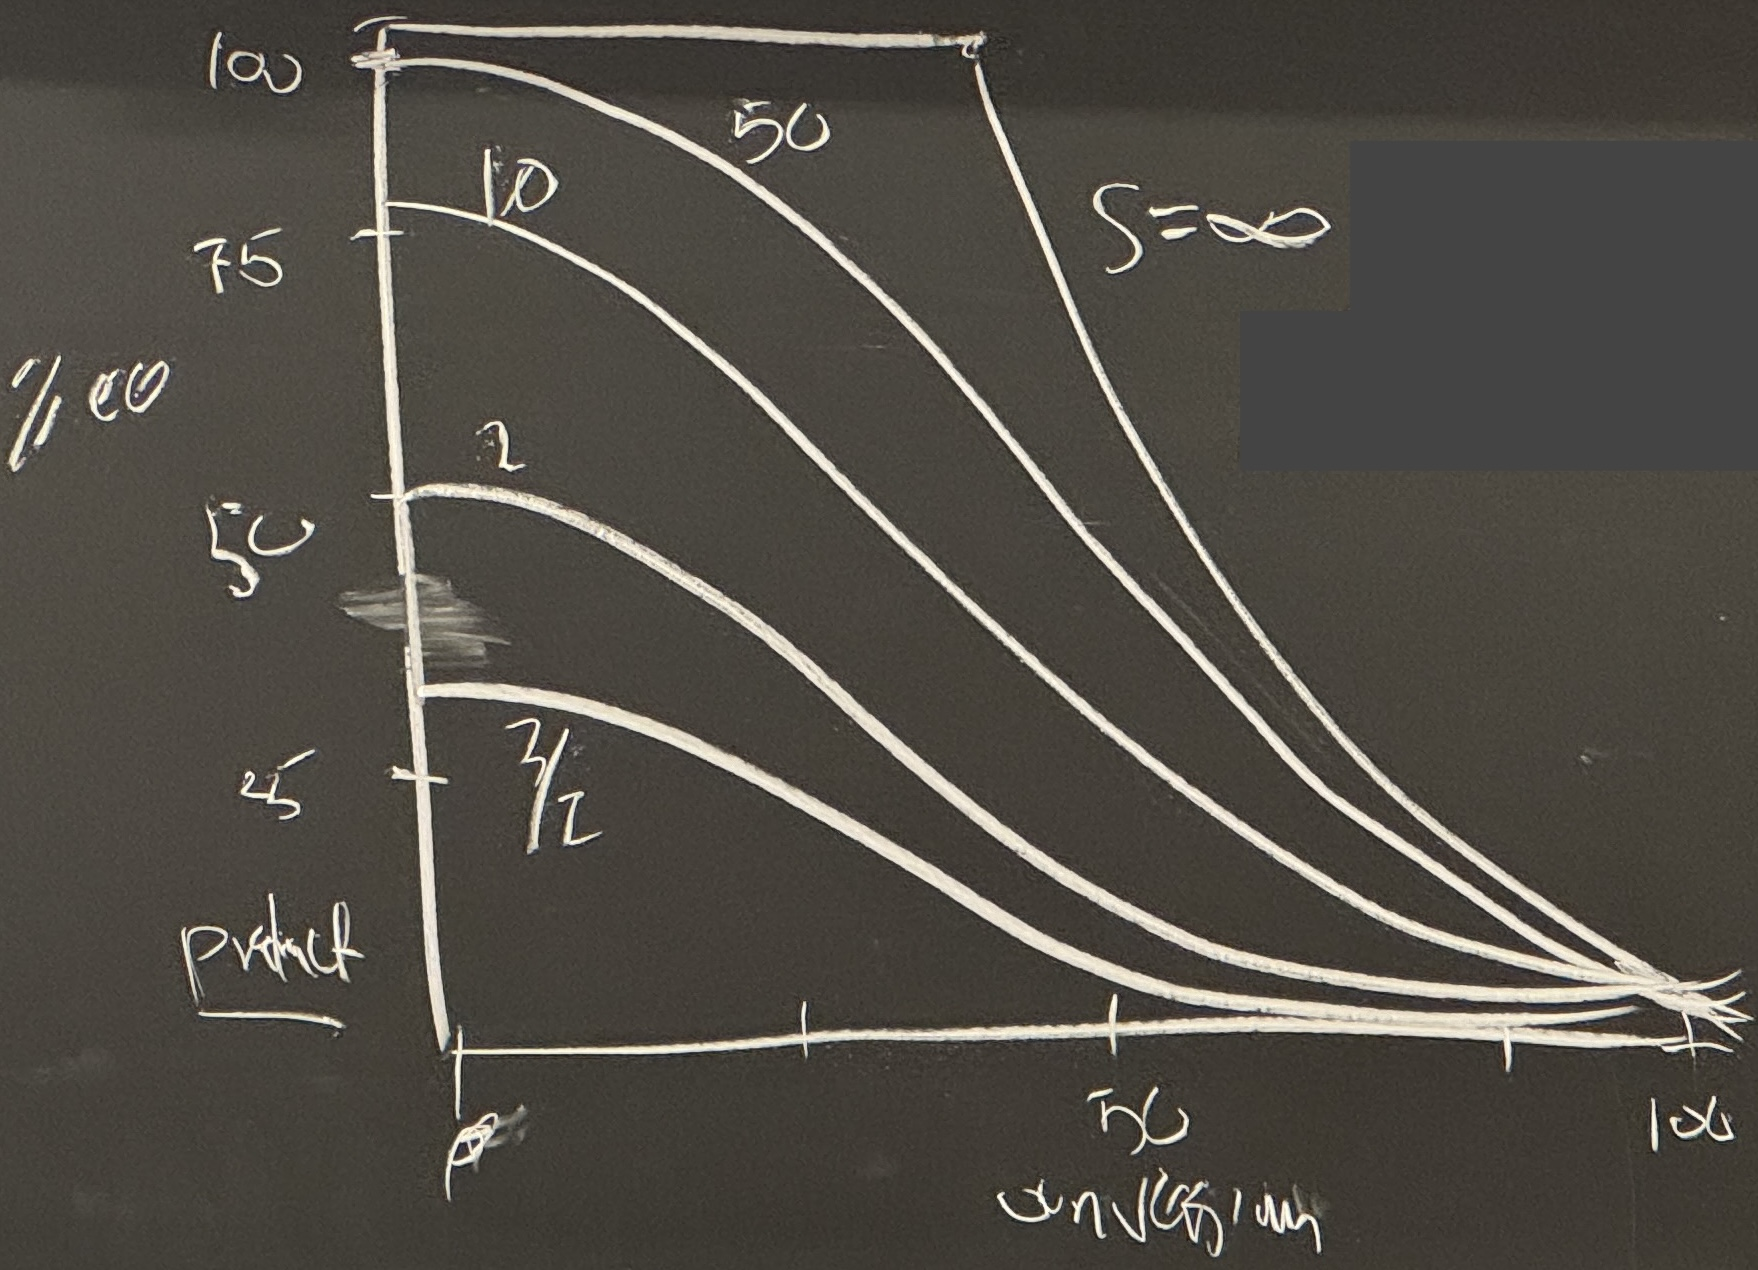
\includegraphics[width=0.43\linewidth]{kinResPee.JPG}
        \caption{Product ee vs. conversion in a catalytic kinetic resolution.}
        \label{fig:kinResPee}
    \end{figure}
    \begin{itemize}
        \item If $S=\infty$, the product will be enantiopure up until we begin converting some of the other enantiomer.
        \item If $S=50$, we start at near-optimal purity, and then our bias will erode.
        \item What this implies is that for the purpose of kinetic resolution of the product, we need very good catalysts.
        \item That's what's remarkable about the Jacobsen catalyst: It's extremely selective for both the starting material \emph{and} product.
    \end{itemize}
    \item Let's now enter into some more complex kinetic regimes.
    \begin{figure}[h!]
        \centering
        \begin{subfigure}[b]{0.25\linewidth}
            \centering
            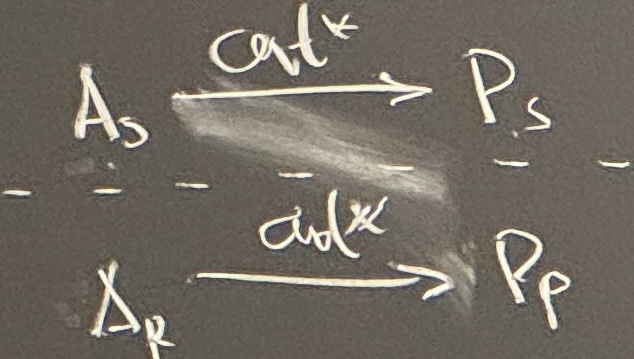
\includegraphics[width=0.7\linewidth]{kinResDyna.JPG}
            \caption{Typical setup.}
            \label{fig:kinResDyna}
        \end{subfigure}
        \begin{subfigure}[b]{0.25\linewidth}
            \centering
            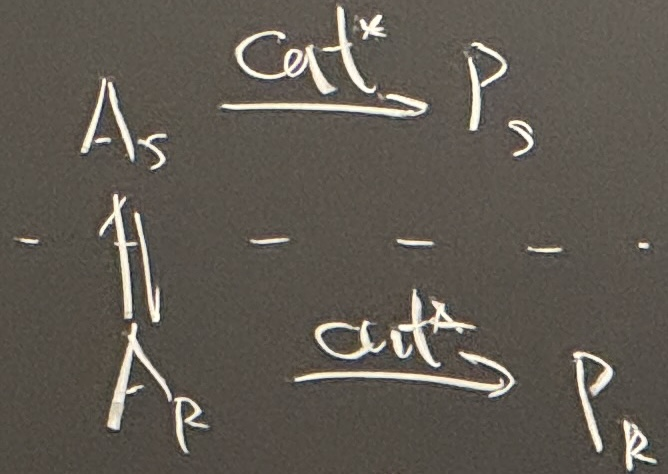
\includegraphics[width=0.65\linewidth]{kinResDynb.JPG}
            \caption{Direct interconversion.}
            \label{fig:kinResDynb}
        \end{subfigure}
        \begin{subfigure}[b]{0.25\linewidth}
            \centering
            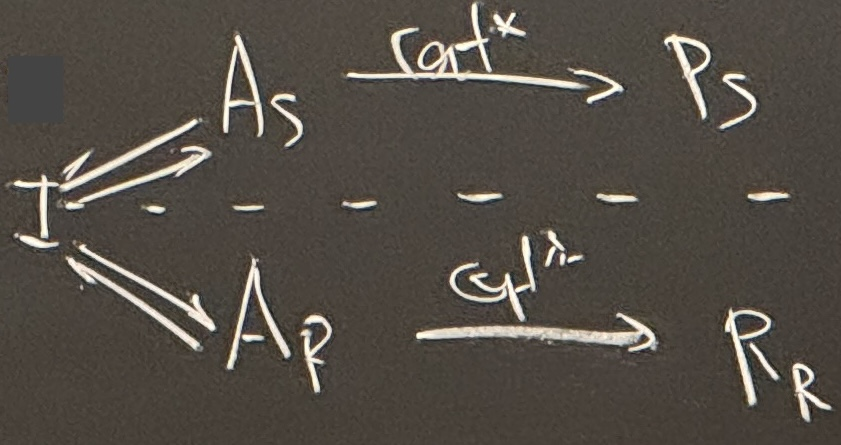
\includegraphics[width=0.7\linewidth]{kinResDync.JPG}
            \caption{Achiral intermediate.}
            \label{fig:kinResDync}
        \end{subfigure}
        \caption{Dynamic kinetic resolution models.}
        \label{fig:kinResDyn}
    \end{figure}
    \pagebreak
    \begin{itemize}
        \item As we've depicted it in Figure \ref{fig:EDcatKinRes}, our starting materials are equal in energy and not interconverting.
        \begin{itemize}
            \item We can conceptualize this scenario as having a mirror plane between our starting materials and products that we \emph{never} cross (Figure \ref{fig:kinResDyna}).
        \end{itemize}
        \item But what about when the starting materials do interconvert?
        \begin{itemize}
            \item There are two ways in which this can happen: We can cross the mirror plane directly (Figure \ref{fig:kinResDynb}), or through an achiral intermediate (Figure \ref{fig:kinResDync}).
        \end{itemize}
        \item The 50\% mass balance limit that is otherwise imposed is now lifted!
        \item Now our catalyst can sample both enantiomers via the epimerization.
        \item \ce{A_S} interconverts with \ce{A_R}, subject to a kinetically selective catalyst.
    \end{itemize}
    \item Enantiomers under fast equilibrium are still under kinetic control, but with 100\% theoretical yield.
    \begin{figure}[h!]
        \centering
        \begin{tikzpicture}[
            every node/.style=black
        ]
            \footnotesize
            \draw (0,4) -- (0,0) -- (6,0);
    
            \draw [dashed] (0.9,1.9) -- (4.7,1.9);
            \draw [->,shorten >=1pt] (1.1,1.9) -- node[fill=white,inner sep=1pt]{$\Delta G^\ddagger_{\ce{S}}$} (1.1,3);
            \draw [->,shorten >=1pt] (4.5,1.9) -- node[fill=white,inner sep=1pt]{$\Delta G^\ddagger_{\ce{R}}$} (4.5,3.8);
    
            \draw [grx,thick] (0.25,0.5) node[below]{\ce{P_S}}
                to[out=0,in=180,looseness=0.6] (1.1,3)
                to[out=0,in=180,out looseness=0.6] (2.1,1.9) node[below]{\ce{A_S}}
                to[out=0,in=180] (2.8,2.2)
                to[out=0,in=180] (3.5,1.9) node[below]{\ce{A_R}}
                to[out=0,in=180,in looseness=0.7] (4.5,3.8)
                to[out=0,in=180,looseness=0.6] (5.75,0.5) node[below]{\ce{P_R}}
            ;
        \end{tikzpicture}
        \caption{Dynamic kinetic resolution energy diagram.}
        \label{fig:EDkinResDyn}
    \end{figure}
    \begin{itemize}
        \item This is known as a \textbf{dynamic kinetic resolution}.
    \end{itemize}
    \item Example dynamic kinetic resolution: Interconversion of chiral $\beta$-ketoesters prior to asymmetric hydrogenation.
    \begin{figure}[H]
        \centering
        \footnotesize
        \schemestart
            \chemfig{Me-[:30](=[2]O)-[:-30](<[6]-[:-30]NHBz)-[:30]CO_2Me}
            \arrow(--.174){->[\tikz{\node[align=center]{(\emph{R})-BINAP-Ru\\\ce{H2}, base}}][$k_\text{fast}$]}[,1.9]
            \chemname{
                \chemfig{Me-[:30](<[2]OH)-[:-30](<[6]-[:-30]NHBz)-[:30]CO_2Me}
            }{\tikz{\node[align=center]{94\% yield\\99\% ee}}}
            \+{,,0.4em}
            \chemname{
                \chemfig{Me-[:30](<:[2]OH)-[:-30](<[6]-[:-30]NHBz)-[:30]CO_2Me}
            }{0.1\% yield}
            \arrow(@c1--){<=>}[-135]
            \chemfig{Me-[:30](-[2]OH)=^[:-30](-[6]-[:-30]NHBz)-[:30]CO_2Me}
            \arrow{<=>}[-45]
            \chemfig{Me-[:30](=[2]O)-[:-30](<:[6]-[:-30]NHBz)-[:30]CO_2Me}
            \arrow(--.176){->[\tikz{\node[align=center]{(\emph{R})-BINAP-Ru\\\ce{H2}, base}}][$k_\text{slow}$]}[,1.9]
            \chemname{
                \chemfig{Me-[:30](<[2]OH)-[:-30](<:[6]-[:-30]NHBz)-[:30]CO_2Me}
            }{5.6\% yield}
            \+{,,0.5em}
            \chemname{
                \chemfig{Me-[:30](<:[2]OH)-[:-30](<:[6]-[:-30]NHBz)-[:30]CO_2Me}
            }{0.5\% yield}
        \schemestop
        \caption{Noyori asymmetric hydrogenation.}
        \label{fig:noyoriAsym}
    \end{figure}
    \begin{itemize}
        \item Consider a racemic sample of $\alpha$-alkylated $\beta$-ketoester.
        \item Subject it to hydrogenation under \textbf{Noyori conditions}.
        \begin{itemize}
            \item Both enantiomeric starting materials may become a \emph{syn} or \emph{anti} diastereomers.
            \item Thus, in principle, you'd get a mess.
        \end{itemize}
        \item Our mess is slightly alleviated by the fact that $\kf/\ks=15$ for the ruthenium-BINAP catalyst.
        \begin{itemize}
            \item This is about \kcal{2} of difference.
            \item However, per Figure \ref{fig:kinResPee}, this S-factor is not great.
        \end{itemize}
        \item Our saving grace is the dynamic nature of this reaction.
        \begin{itemize}
            \item When we actually run the experiment, we get fast enolization and interconversion through an achiral intermediate because of the base\footnote{It appears from the paper that there may not be a base; this may just be keto-enol tautomerization.} in solution and the acidic $\alpha$-proton.
            \item Indeed, if the rate of enolization/racemation is denoted by $k_\text{rac}$, we have $k_\text{rac}/\kf\approx 100$!
        \end{itemize}
        \item Thus, we get 94\% yield of one stereoisomer in 99\% ee.
        \item Reference: \textcite{bib:noyoriAsym}.
        \begin{itemize}
            \item See Table 3, Figure 19, and the associated discussions.
            \item The whole paper is a good review of this chemistry, though.
        \end{itemize}
    \end{itemize}
    \item \textbf{Noyori asymmetric hydrogenation}: The asymmetric hydrogenation of a ketone using a homochiral ruthenium-BINAP catalyst, hydrogen gas, and a base.
    \item A related kinetic selectivity: Curtin-Hammett kinetics.
    \begin{figure}[h!]
        \centering
        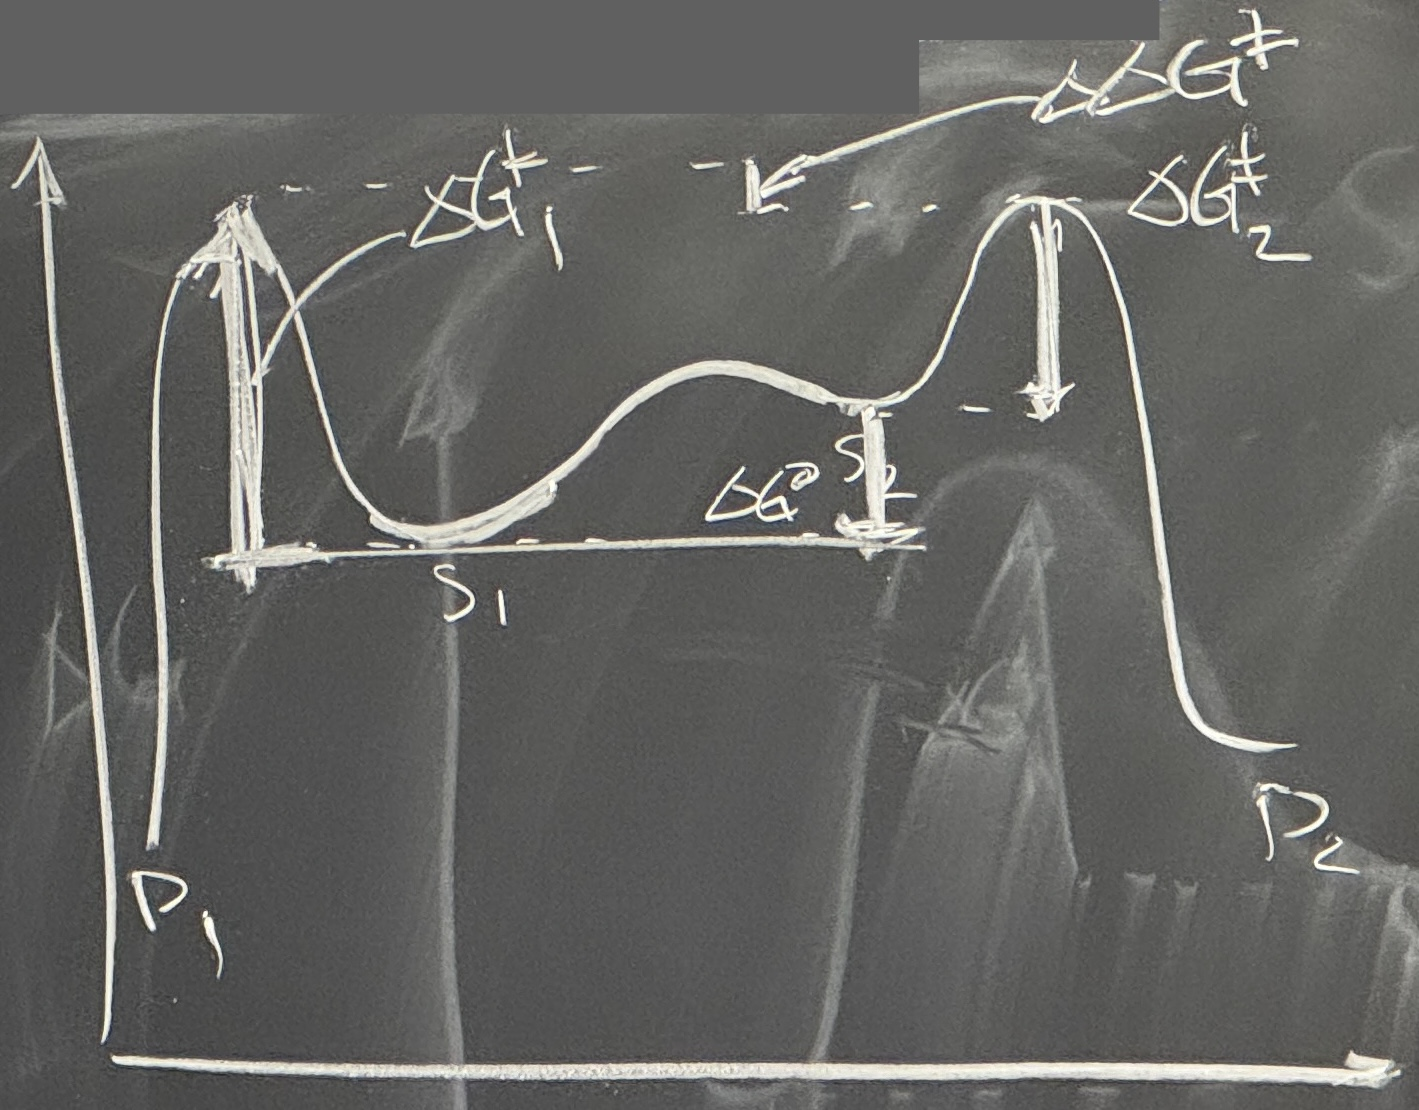
\includegraphics[width=0.4\linewidth]{CHselectDeriv.JPG}
        \caption{Curtin-Hammett selectivity derivation.}
        \label{fig:CHselectDeriv}
    \end{figure}
    \begin{itemize}
        \item Instead of (\emph{R})- and (\emph{S})-enantiomers, which rigorously have the same energy, we can consider other interconverting species with different energies.
        \item We can quantitate --- with rate laws --- the formation of the products.
        \begin{align*}
            \dv{\cnc{P1}}{t} &= k_1\cnc{S1}&
            \dv{\cnc{P2}}{t} &= k_2\cnc{S2}
        \end{align*}
        \item Then taking a ratio gives
        \begin{equation*}
            \dv{\cnc{P1}}{\cnc{P2}} = \frac{k_1\cnc{S1}}{k_2\cnc{S2}}
        \end{equation*}
        \item Note that
        \begin{equation*}
            \frac{\cnc{S1}}{\cnc{S2}} = \Keq
        \end{equation*}
        so
        \begin{equation*}
            \dv{\cnc{P1}}{\cnc{P2}} = \frac{k_1}{k_2}\Keq
        \end{equation*}
        \item Thus, with Arrhenius,
        \begin{equation*}
            \dv{\cnc{P1}}{\cnc{P2}} = \frac{\e[-\Delta G^\ddagger_2/RT]}{\e[-\Delta G^\ddagger_1/RT]}\e[-\Delta G^\circ/RT]
            = \e[(\Delta G^\ddagger_1-\Delta G^\ddagger_2-\Delta G^\circ)/RT]
        \end{equation*}
        \item And then referencing Figure \ref{fig:CHselectDeriv}, we can see pictorially that
        \begin{equation*}
            \Delta G^\ddagger_1-\Delta G^\ddagger_2-\Delta G^\circ = \Delta\Delta G^\ddagger
        \end{equation*}
        \item Thus, 
        \begin{equation*}
            \dv{\cnc{P1}}{\cnc{P2}} = \e[\Delta\Delta G^\ddagger/RT]
        \end{equation*}
        if we have a fast equilibrium \ce{S1 <=> S2} (10 times faster than \ce{P1} or \ce{P2} formation).
        \item Essentially, if we have this fast starting equilibrium, then the product ratio is under kinetic control.
    \end{itemize}
    \item Now suppose we drop \ce{S2} down in free energy and leave the rest of the diagram unperturbed.
    \begin{itemize}
        \item This change in one variable is compensated for by a change in the other variable, and we remain under kinetic control.
    \end{itemize}
    \item Alex briefly discusses kinetic quench.
    \item Curtin-Hammett example 1 (Figure \ref{fig:CHscenarioa}).
    \begin{itemize}
        \item \ce{P1} is kinetically favored.
        \item $\cnc{S1}>\cnc{S2}$.
        \item Here, the \ce{S1}/\ce{S2} ratio is irrelevant to product formation. This is "invisible" C/H kinetics. Mathematically,
        \begin{equation*}
            \frac{\cnc{S1}}{\cnc{S2}} \neq \frac{\cnc{P1}}{\cnc{P2}}
        \end{equation*}
    \end{itemize}
    \item Curtin-Hammett example 2 (Figure \ref{fig:CHscenariob}).
    \begin{itemize}
        \item \ce{P1} is kinetically favored.
        \item $\cnc{S1}<\cnc{S2}$.
        \item This is "classic" C/H kinetics.
        \item Great example of this in \textcite{bib:CHexample}.
        \item This scenario is actually pretty common.
    \end{itemize}
    \item Curtin-Hammett example 3 (Figure \ref{fig:CHscenarioc}).
    \begin{itemize}
        \item Here, $\Delta G^\ddagger_1=\Delta G^\ddagger_2$.
        \item This scenario is pretty uncommon, but it is possible.
        \item In this case, the equilibrium ratio \emph{does} reflect the product ratio.
    \end{itemize}
    \item Takeaway: It is far more likely that your equilibrium ratio of intermediates has no bearing on your ratio of products.
\end{itemize}



\section{Exam 2 Review Sheet}
\begin{itemize}
    \item \marginnote{12/4:}Noncovalent interactions.
    \begin{itemize}
        \item Quadrupoles preferentially bind hard, positively charged ions.
        \item The strongest hydrogen bonds have short bond lengths and are nearly linear; vice versa for weak.
        \item There is an energetic penalty to mixing polar and nonpolar solvents. The penalty is mostly entropic, because putting a hydrophobic link in the water disrupts the water's ability to randomly hydrogen bond to itself. Less \ce{H}-bonding means more ordered, less entropic water.
    \end{itemize}
    \item Transition states are first-order saddle points on a hypersurface defined by vibrational DOFs.
    \begin{itemize}
        \item $\Delta G=-RT\ln\Keq$.
        \item $\Delta G^\ddagger=-RT\ln k$.
        \item $\Delta\Delta G^\ddagger=-RT\ln(k_{\ce{A}}/k_{\ce{B}})$
    \end{itemize}
    \item \textbf{van't Hoff analysis}: Experimental determination of $\Delta H^\circ$ and $\Delta S^\circ$.
    \begin{align*}
        -RT\ln\Keq &= \Delta H^\circ-T\Delta S^\circ\\
        R\ln\Keq &= -\Delta H^\circ\left( \frac{1}{T} \right)+\Delta S^\circ
    \end{align*}
    \item Fragmentations give \kcal{9}, or \eu{30} at \SI{300}{\kelvin}.
    \item Transition state theory.
    \begin{itemize}
        \item General form.
        \begin{equation*}
            \ce{A <=>[$K^\ddagger$] [TS] ->[$k^\ddagger$] B}
        \end{equation*}
        \item Postulates.
        \begin{enumerate}
            \item Activated complex is in quasi-equilibrium with starting material.
            \item Any molecule that makes its way to the transition state will then proceed onto the product barrierlessly ($\kappa=1$).
        \end{enumerate}
        \item The number of times a starting material appears in the TS is it's order in the rate law.
        \item Eyring equation:
        \begin{equation*}
            k = \kappa\left( \frac{\kB T}{h} \right)\e[-\Delta G^\ddagger/RT]
        \end{equation*}
        \begin{itemize}
            \item Linearization (for experimental determination of $\Delta H^\ddagger$ and $\Delta S^\ddagger$):
            \begin{equation*}
                \ln(\frac{kh}{\kappa\kB T}) = -\frac{\Delta H^\ddagger}{R}\left( \frac{1}{T} \right)+\frac{\Delta S^\ddagger}{R}
            \end{equation*}
        \end{itemize}
        \item Hammond postulate.
    \end{itemize}
    \item Isotope effects.
    \begin{itemize}
        \item QMech foundation:
        \begin{align*}
            E_n &= h\nu\left( n+\frac{1}{2} \right)&
            \nu &= \frac{1}{2\pi}\sqrt{\frac{k}{\mu}}
        \end{align*}
        \item \ce{C-D} lower by \kcal{1.5}.
        \item Equilibrium isotope effect:
        \begin{equation*}
            \frac{K_{\ce{H}}}{K_{\ce{D}}}
        \end{equation*}
        \item \ce{C-D} bonds hold onto their electrons more tightly.
        \item Kinetic isotope effect.
        \begin{equation*}
            \KIE = \frac{k_{\ce{H}}}{k_{\ce{D}}}
        \end{equation*}
        \item Asymmetric stretch is the reaction coordinate.
        \begin{itemize}
            \item Symmetric stretch is the important orthogonal vector.
            \item Under thermoneutral conditions with identical atoms on either side, $\KIE=\max$ because the symmetric stretch has no isotopic sensitivity.
        \end{itemize}
        \item Bent transition states have more contributions from bending mode isotopic sensitivities, but smaller overall sensitivities (1.5-3.5).
        \item Quantum tunnelling can give anomously large KIEs.
        \item Secondary isotope effects at the $\alpha$-position largely governed by out-of-plane bending modes.
        \begin{itemize}
            \item Going to a slacker potential: Normal $2^\circ$ KIE.
            \item Going to a stiffer potential: Inverse $2^\circ$ KIE.
        \end{itemize}
        \item Secondary isotope effects at the $\beta$-position governed by hyperconjugation, or actually primary because involved (e.g., E\textsubscript{2}).
        \item Experimental determination.
        \begin{itemize}
            \item Independent absolute rate measurement.
            \item Intramolecular competition experiment.
            \begin{itemize}
                \item Correction: If
                \begin{align*}
                    C &:= \frac{\cnc{P_H}}{\cnc[0]{SM_H}}&
                    R &:= \left( \frac{\cnc{SM_D}}{\cnc{SM_H}} \right)_t&
                    R_0 &:= \left( \frac{\cnc{SM_D}}{\cnc{SM_H}} \right)_0
                \end{align*}
                then
                \begin{equation*}
                    \KIE = \frac{k_{\ce{H}}}{k_{\ce{D}}}
                    = \frac{\ln(1-C)}{\ln\left[ (1-C)\cdot\frac{R}{R_0} \right]}
                \end{equation*}
            \end{itemize}
            \item Intramolecular competition can probe post-rate-determining steps.
            \begin{itemize}
                \item Extract KIE from the product ratio at \emph{any} conversion.
            \end{itemize}
        \end{itemize}
        \item Heavy-atom KIEs.
        \begin{itemize}
            \item Extracted at high conversions.
            \item Choose a reference atom, take NMRs at high conversion, plug into conversion formula to get KIEs.
            \item Can tell you what sites are involved in the RDS!
            \item Conversion-\emph{dependent} isotopic enrichment is affiliated with the RDS.
            \item Conversion-\emph{independent} isotopic enrichment is affiliated with post-RDS steps.
        \end{itemize}
    \end{itemize}
    \item Rate laws.
    \begin{itemize}
        \item Zeroeth-order, first-order, and second-order integrated rate laws.
        \item $\kobs$ vs. swamping concentrations to determine $k$.
        \item SSA.
        \begin{itemize}
            \item If \ce{A} is more stable than \ce{B}, the SSA is valid.
            \item If \ce{I} is depleted faster than it is formed, the SSA is valid.
        \end{itemize}
        \item QEA.
        \begin{itemize}
            \item Only valid when $k_{-1}>k_2$.
        \end{itemize}
        \item Limiting cases.
        \item The saturation regime.
        \item Defining the total concentration of the catalyst is often useful.
        \item Michaelis-Menten kinetics.
        \item Blackmond's work.
        \begin{itemize}
            \item Same-excess experiment and visual overlay.
            \item Different excess experiment.
        \end{itemize}
    \end{itemize}
    \item Kinetic resolution.
    \begin{itemize}
        \item Relations between conversion and ee.
        \item Dynamic kinetic resolution: Going through an intermediate or other interconversion.
        \item Curtin-Hammett kinetics.
    \end{itemize}
\end{itemize}




\end{document}